% Options for packages loaded elsewhere
\PassOptionsToPackage{unicode}{hyperref}
\PassOptionsToPackage{hyphens}{url}
%
\documentclass[
]{article}
\usepackage{amsmath,amssymb}
\usepackage{iftex}
\ifPDFTeX
  \usepackage[T1]{fontenc}
  \usepackage[utf8]{inputenc}
  \usepackage{textcomp} % provide euro and other symbols
\else % if luatex or xetex
  \usepackage{unicode-math} % this also loads fontspec
  \defaultfontfeatures{Scale=MatchLowercase}
  \defaultfontfeatures[\rmfamily]{Ligatures=TeX,Scale=1}
\fi
\usepackage{lmodern}
\ifPDFTeX\else
  % xetex/luatex font selection
\fi
% Use upquote if available, for straight quotes in verbatim environments
\IfFileExists{upquote.sty}{\usepackage{upquote}}{}
\IfFileExists{microtype.sty}{% use microtype if available
  \usepackage[]{microtype}
  \UseMicrotypeSet[protrusion]{basicmath} % disable protrusion for tt fonts
}{}
\makeatletter
\@ifundefined{KOMAClassName}{% if non-KOMA class
  \IfFileExists{parskip.sty}{%
    \usepackage{parskip}
  }{% else
    \setlength{\parindent}{0pt}
    \setlength{\parskip}{6pt plus 2pt minus 1pt}}
}{% if KOMA class
  \KOMAoptions{parskip=half}}
\makeatother
\usepackage{xcolor}
\usepackage[margin=1in]{geometry}
\usepackage{color}
\usepackage{fancyvrb}
\newcommand{\VerbBar}{|}
\newcommand{\VERB}{\Verb[commandchars=\\\{\}]}
\DefineVerbatimEnvironment{Highlighting}{Verbatim}{commandchars=\\\{\}}
% Add ',fontsize=\small' for more characters per line
\usepackage{framed}
\definecolor{shadecolor}{RGB}{248,248,248}
\newenvironment{Shaded}{\begin{snugshade}}{\end{snugshade}}
\newcommand{\AlertTok}[1]{\textcolor[rgb]{0.94,0.16,0.16}{#1}}
\newcommand{\AnnotationTok}[1]{\textcolor[rgb]{0.56,0.35,0.01}{\textbf{\textit{#1}}}}
\newcommand{\AttributeTok}[1]{\textcolor[rgb]{0.13,0.29,0.53}{#1}}
\newcommand{\BaseNTok}[1]{\textcolor[rgb]{0.00,0.00,0.81}{#1}}
\newcommand{\BuiltInTok}[1]{#1}
\newcommand{\CharTok}[1]{\textcolor[rgb]{0.31,0.60,0.02}{#1}}
\newcommand{\CommentTok}[1]{\textcolor[rgb]{0.56,0.35,0.01}{\textit{#1}}}
\newcommand{\CommentVarTok}[1]{\textcolor[rgb]{0.56,0.35,0.01}{\textbf{\textit{#1}}}}
\newcommand{\ConstantTok}[1]{\textcolor[rgb]{0.56,0.35,0.01}{#1}}
\newcommand{\ControlFlowTok}[1]{\textcolor[rgb]{0.13,0.29,0.53}{\textbf{#1}}}
\newcommand{\DataTypeTok}[1]{\textcolor[rgb]{0.13,0.29,0.53}{#1}}
\newcommand{\DecValTok}[1]{\textcolor[rgb]{0.00,0.00,0.81}{#1}}
\newcommand{\DocumentationTok}[1]{\textcolor[rgb]{0.56,0.35,0.01}{\textbf{\textit{#1}}}}
\newcommand{\ErrorTok}[1]{\textcolor[rgb]{0.64,0.00,0.00}{\textbf{#1}}}
\newcommand{\ExtensionTok}[1]{#1}
\newcommand{\FloatTok}[1]{\textcolor[rgb]{0.00,0.00,0.81}{#1}}
\newcommand{\FunctionTok}[1]{\textcolor[rgb]{0.13,0.29,0.53}{\textbf{#1}}}
\newcommand{\ImportTok}[1]{#1}
\newcommand{\InformationTok}[1]{\textcolor[rgb]{0.56,0.35,0.01}{\textbf{\textit{#1}}}}
\newcommand{\KeywordTok}[1]{\textcolor[rgb]{0.13,0.29,0.53}{\textbf{#1}}}
\newcommand{\NormalTok}[1]{#1}
\newcommand{\OperatorTok}[1]{\textcolor[rgb]{0.81,0.36,0.00}{\textbf{#1}}}
\newcommand{\OtherTok}[1]{\textcolor[rgb]{0.56,0.35,0.01}{#1}}
\newcommand{\PreprocessorTok}[1]{\textcolor[rgb]{0.56,0.35,0.01}{\textit{#1}}}
\newcommand{\RegionMarkerTok}[1]{#1}
\newcommand{\SpecialCharTok}[1]{\textcolor[rgb]{0.81,0.36,0.00}{\textbf{#1}}}
\newcommand{\SpecialStringTok}[1]{\textcolor[rgb]{0.31,0.60,0.02}{#1}}
\newcommand{\StringTok}[1]{\textcolor[rgb]{0.31,0.60,0.02}{#1}}
\newcommand{\VariableTok}[1]{\textcolor[rgb]{0.00,0.00,0.00}{#1}}
\newcommand{\VerbatimStringTok}[1]{\textcolor[rgb]{0.31,0.60,0.02}{#1}}
\newcommand{\WarningTok}[1]{\textcolor[rgb]{0.56,0.35,0.01}{\textbf{\textit{#1}}}}
\usepackage{graphicx}
\makeatletter
\def\maxwidth{\ifdim\Gin@nat@width>\linewidth\linewidth\else\Gin@nat@width\fi}
\def\maxheight{\ifdim\Gin@nat@height>\textheight\textheight\else\Gin@nat@height\fi}
\makeatother
% Scale images if necessary, so that they will not overflow the page
% margins by default, and it is still possible to overwrite the defaults
% using explicit options in \includegraphics[width, height, ...]{}
\setkeys{Gin}{width=\maxwidth,height=\maxheight,keepaspectratio}
% Set default figure placement to htbp
\makeatletter
\def\fps@figure{htbp}
\makeatother
\setlength{\emergencystretch}{3em} % prevent overfull lines
\providecommand{\tightlist}{%
  \setlength{\itemsep}{0pt}\setlength{\parskip}{0pt}}
\setcounter{secnumdepth}{-\maxdimen} % remove section numbering
\ifLuaTeX
  \usepackage{selnolig}  % disable illegal ligatures
\fi
\IfFileExists{bookmark.sty}{\usepackage{bookmark}}{\usepackage{hyperref}}
\IfFileExists{xurl.sty}{\usepackage{xurl}}{} % add URL line breaks if available
\urlstyle{same}
\hypersetup{
  pdftitle={Supplementary Material},
  hidelinks,
  pdfcreator={LaTeX via pandoc}}

\title{Supplementary Material}
\author{}
\date{\vspace{-2.5em}2022-10-27}

\begin{document}
\maketitle

The present document contains details about the data-analysis for the
paper entitled: ``The assessment of presence and performance in an AR
environment for motor imitation learning: a case-study on violinists.''
Authors: Adriaan Campo, Aleksandra Michałko, Bavo Van Kerrebroeck, Boris
Stajic, Maja Pokric, Marc Leman. Basically, the paper tests a violin
playback system. The violinist's task is to play in synchrony with the
principal violinist of an orchestra (represented as an avatar). The
playback system provides the audio, in addition to a 2D or 3D avatar via
a Hololens. The focus is mainly on the effect due to the experimental
conditions of a 2D or 3D playback.

\hypertarget{workflow}{%
\section{Workflow}\label{workflow}}

Figure 1 shows two statistical workflows. The upper workflow on top is
about the biomechanical metrics from motion capture (here called:
procustus and sparc, instead of PD and dSI as in the paper). Each metric
represents differences between the violinist and the avatar, summarized
over time. These values are used as response in regression models,
whereas conditions, participants and trial are used as predictors.
Model\_1 and model\_2 are similar models except that in model\_2
\texttt{difficulty} is added in interaction with condition. The lower
workflow is about the behavioral metrics of the questionnaires. We have
3 presence questionnaires. Model\_3 and model\_4 are similar models
except that in model\_4 \texttt{procustus} is added in interaction with
condition.

In the upper workflow, we start with a comparison of model\_1 and
model\_2 to test whether \texttt{difficulty} should be added to the
model. We then perform a more detailed diagnostics of the best model, as
well as a contrast analysis of condition and trials. In the lower
workflow, we start with a comparison of model\_3 and model\_4 to test
whether \texttt{procustus} should be added to the model. We then proceed
with a more detailed diagnostics of the best model, as well as a
contrast analysis of conditions.

\begin{figure}
\centering
\includegraphics{FiguresPaper/StatisticPath1.png}
\caption{Statistical path}
\end{figure}

The workflows hold a scheme for testing the work hypothesis, as shown in
figure 2:

Hypothesis 1. Students will show better violin performance in the 3D
condition compared to the 2D condition:

\begin{itemize}
\item
  1.1. Similarity between virtual teachers' and students' bow movement
  is higher .
\item
  1.2. Movement smoothness is higher
\end{itemize}

Hypothesis 2. Learning effectiveness of violin performance will be
higher in the 3D condition compared to the 2D condition.

Hypothesis 3. The 3D condition will induce a higher level of presence
compared to the 2D condition:

\begin{itemize}
\item
  3.1. ``physical presence'' will be higher
\item
  3.2. ``social presence'' will be higher
\end{itemize}

Hypothesis 4. The level of presence in AR influences students' violin
performance.

\begin{figure}
\centering
\includegraphics{FiguresPaper/StatisticPath2.png}
\caption{Hypothesis testing}
\end{figure}

In hypothesis 1, we first compare model\_1 and model\_2 and focus on the
contrast analysis of the best model. This analysis will tell us the
differences between conditions. In hypothesis 2, we expand our contrast
analysis by comparing conditions and trials. In hypothesis 3, we do a
contrast analysis of model\_3.\\
In hypothesis 4 we test whether the procustus metric might be a relevant
predictor variable.

\hypertarget{power-analysis}{%
\section{Power Analysis}\label{power-analysis}}

A retrospective power analysis of the setup shown in Figure 3 reveals
that 11 participants and 4 repeated measures has sufficient power when
Cohen's D is \textgreater{} 0.6. To show that, we used a hierarchical
statistical model with 2 conditions, and with participants and trials
modeled as groups for which we assumed a standard deviation of 0.25 and
0.1, respectively. We tested Cohen's D from 0 to 0.6, and a number of
participants from 5 to 30. For each dot in the graph below (e.g.~D =
0.5, number of participants = 20) we simulated 500 models and tested
whether the contrast of conditions has a probability mass of
\textgreater= .95. The proportion of yes (versus no) is presented as
power (in \%). The results show that 11 participants have enough power
(\textgreater{} 80\%) when Cohen's D is \textgreater{} 0.6, meaning that
there is \textless20\% to miss an effect when there is in fact an effect
(= false negative). In our models, we observe that the calibrated models
have D \textgreater{} 0.8 (for the models: see below).

\begin{figure}
\centering
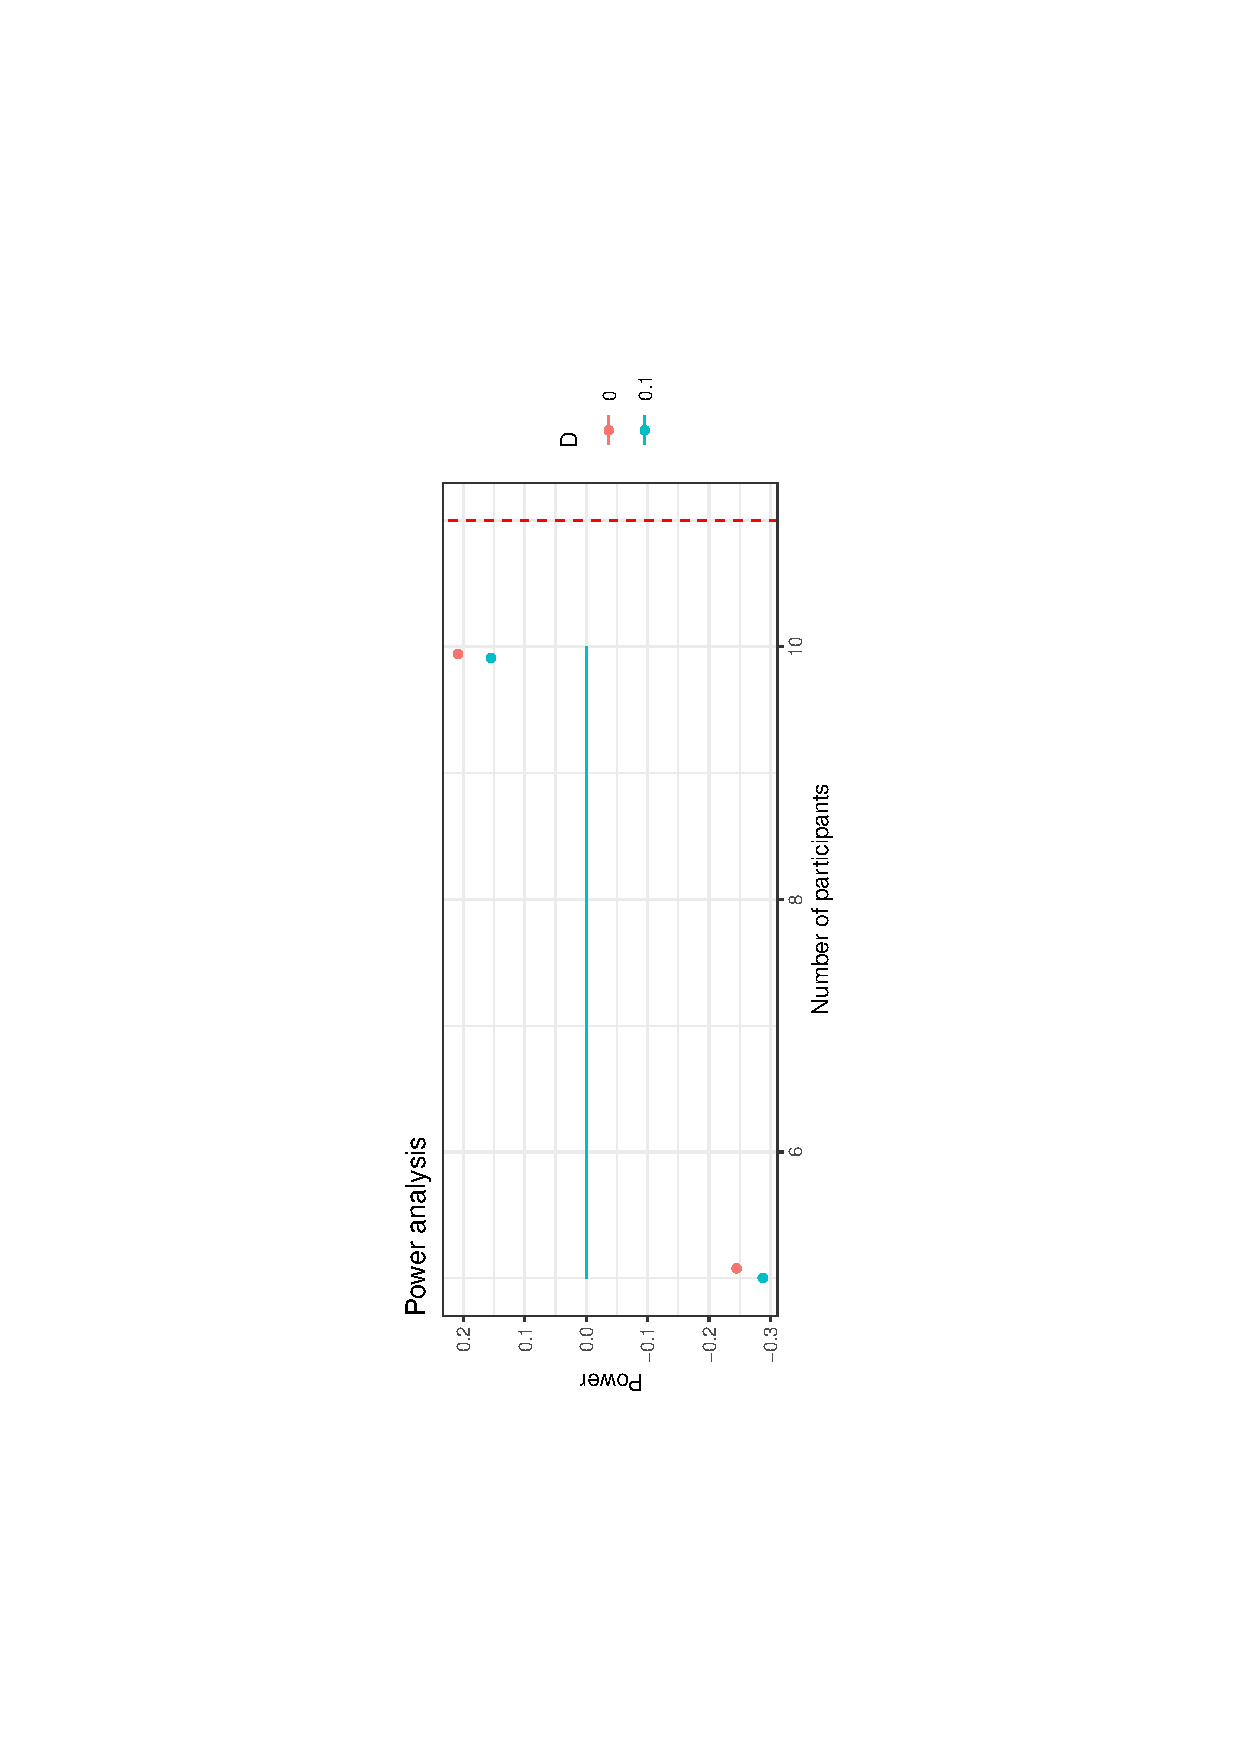
\includegraphics{FiguresPaper/PowerAnalysis03.png}
\caption{Retrospective power analysis. The dotted vertical line marks 11
participants, as used in thep present study}
\end{figure}

\hypertarget{data}{%
\section{Data}\label{data}}

The first box in the workflow shown in Figure 1 is about data. We use
one dataset for all models. The data variables are listed below:

\begin{Shaded}
\begin{Highlighting}[]
\FunctionTok{load}\NormalTok{(}\AttributeTok{file =} \StringTok{"Data.RData"}\NormalTok{)}
\FunctionTok{str}\NormalTok{(Data)}
\end{Highlighting}
\end{Shaded}

\begin{verbatim}
## 'data.frame':    88 obs. of  16 variables:
##  $ participant             : Factor w/ 11 levels "1","2","3","4",..: 1 1 1 1 1 1 1 1 10 10 ...
##  $ condition               : Factor w/ 2 levels "1","2": 1 1 1 1 2 2 2 2 1 1 ...
##  $ trial                   : Factor w/ 4 levels "1","2","3","4": 1 2 3 4 1 2 3 4 1 2 ...
##  $ response1M_procustus    : num  0.5448 0.0614 0.1508 -0.076 -0.0535 ...
##  $ response0M_procustus    : num  1.319 0.835 0.925 0.698 0.43 ...
##  $ response1M_sparc        : num  -0.0896 -0.1224 -0.1035 -0.048 0.1661 ...
##  $ response0M_sparc        : num  11.2 11.1 11.1 11.2 11.1 ...
##  $ WPQ                     : num  4.07 3.93 4.04 4.11 5 ...
##  $ MPQS                    : num  2.8 3.2 3 2 4 5.2 4.6 4.8 4.8 4 ...
##  $ MPQP                    : num  3.4 3 2.8 2.8 4.2 6 5.2 6 3.8 4.4 ...
##  $ Difficulty              : num [1:88, 1] -0.203 -0.993 -1.586 -1.191 -0.5 ...
##  $ log_response0M_procustus: num  0.2766 -0.18 -0.0784 -0.3598 -0.8436 ...
##  $ log_response1M_procustus: num  -0.607 -2.79 -1.892 NA NA ...
##  $ log_response0M_sparc    : num  2.41 2.41 2.41 2.42 2.4 ...
##  $ log_response1M_sparc    : num  NA NA NA NA -1.8 ...
##  $ difficulty_s            : num [1:88, 1] -0.203 -0.993 -1.586 -1.191 -0.5 ...
\end{verbatim}

\begin{Shaded}
\begin{Highlighting}[]
\FunctionTok{head}\NormalTok{(Data)}
\end{Highlighting}
\end{Shaded}

\begin{verbatim}
##   participant condition trial response1M_procustus response0M_procustus
## 1           1         1     1           0.54477643            1.3185912
## 2           1         1     2           0.06143131            0.8352461
## 3           1         1     3           0.15080784            0.9246226
## 4           1         1     4          -0.07599130            0.6978235
## 5           1         2     1          -0.05350941            0.4301667
## 6           1         2     2          -0.07670672            0.4069694
##   response1M_sparc response0M_sparc      WPQ MPQS MPQP Difficulty
## 1      -0.08964702         11.15673 4.074074  2.8  3.4 -0.2033571
## 2      -0.12239219         11.12399 3.925926  3.2  3.0 -0.9932761
## 3      -0.10351349         11.14287 4.037037  3.0  2.8 -1.5857154
## 4      -0.04796922         11.19841 4.111111  2.0  2.8 -1.1907559
## 5       0.16611262         11.06114 5.000000  4.0  4.2 -0.4995767
## 6       0.16967439         11.06470 5.518519  5.2  6.0  0.6359318
##   log_response0M_procustus log_response1M_procustus log_response0M_sparc
## 1               0.27656388               -0.6073798             2.412043
## 2              -0.18002891               -2.7898356             2.409104
## 3              -0.07836964               -1.8917489             2.410800
## 4              -0.35978914                       NA             2.415772
## 5              -0.84358250                       NA             2.403438
## 6              -0.89901733                       NA             2.403760
##   log_response1M_sparc difficulty_s
## 1                   NA   -0.2033571
## 2                   NA   -0.9932761
## 3                   NA   -1.5857154
## 4                   NA   -1.1907559
## 5            -1.795089   -0.4995767
## 6            -1.773874    0.6359318
\end{verbatim}

\begin{Shaded}
\begin{Highlighting}[]
\FunctionTok{summary}\NormalTok{(Data)}
\end{Highlighting}
\end{Shaded}

\begin{verbatim}
##   participant condition trial  response1M_procustus response0M_procustus
##  1      : 8   1:44      1:22   Min.   :-0.279936    Min.   :0.3399      
##  2      : 8   2:44      2:23   1st Qu.:-0.088432    1st Qu.:0.5096      
##  3      : 8             3:21   Median : 0.008438    Median :0.6013      
##  4      : 8             4:22   Mean   : 0.056997    Mean   :0.6749      
##  5      : 8                    3rd Qu.: 0.111951    3rd Qu.:0.8061      
##  6      : 8                    Max.   : 1.247398    Max.   :2.0212      
##  (Other):40                                                             
##  response1M_sparc    response0M_sparc      WPQ             MPQS      
##  Min.   :-0.640874   Min.   :10.25    Min.   :3.852   Min.   :1.000  
##  1st Qu.:-0.085935   1st Qu.:11.00    1st Qu.:4.444   1st Qu.:2.600  
##  Median : 0.005891   Median :11.17    Median :4.907   Median :3.200  
##  Mean   :-0.018900   Mean   :11.10    Mean   :4.891   Mean   :3.151  
##  3rd Qu.: 0.090802   3rd Qu.:11.28    3rd Qu.:5.259   3rd Qu.:3.800  
##  Max.   : 0.309727   Max.   :11.56    Max.   :6.222   Max.   :5.200  
##                                       NA's   :2       NA's   :2      
##       MPQP          Difficulty.V1     log_response0M_procustus
##  Min.   :2.000   Min.   :-2.0300448   Min.   :-1.0792         
##  1st Qu.:3.400   1st Qu.:-0.7217415   1st Qu.:-0.6742         
##  Median :4.200   Median :-0.0799323   Median :-0.5086         
##  Mean   :3.991   Mean   : 0.0000000   Mean   :-0.4594         
##  3rd Qu.:4.600   3rd Qu.: 0.7470142   3rd Qu.:-0.2156         
##  Max.   :6.000   Max.   : 2.2651397   Max.   : 0.7037         
##  NA's   :2                                                    
##  log_response1M_procustus log_response0M_sparc log_response1M_sparc
##  Min.   :-6.2271          Min.   :2.328        Min.   :-5.680      
##  1st Qu.:-3.3151          1st Qu.:2.398        1st Qu.:-3.371      
##  Median :-2.6006          Median :2.413        Median :-2.401      
##  Mean   :-2.4148          Mean   :2.407        Mean   :-2.657      
##  3rd Qu.:-1.5421          3rd Qu.:2.423        3rd Qu.:-1.777      
##  Max.   : 0.2211          Max.   :2.447        Max.   :-1.172      
##  NA's   :41                                    NA's   :43          
##    difficulty_s.V1   
##  Min.   :-2.0300448  
##  1st Qu.:-0.7217415  
##  Median :-0.0799323  
##  Mean   : 0.0000000  
##  3rd Qu.: 0.7470142  
##  Max.   : 2.2651397  
## 
\end{verbatim}

It is of interest to show the differences between non-calibrated and
calibrated metrics, all obtained by taking the median of the data points
(summarizing time).

\begin{Shaded}
\begin{Highlighting}[]
\FunctionTok{load}\NormalTok{(}\AttributeTok{file =} \StringTok{"Data.RData"}\NormalTok{)}
\FunctionTok{library}\NormalTok{(ggplot2)}
\FunctionTok{library}\NormalTok{(patchwork)}
\NormalTok{p1 }\OtherTok{\textless{}{-}} \FunctionTok{ggplot}\NormalTok{(Data) }\SpecialCharTok{+}
  \FunctionTok{geom\_point}\NormalTok{(}\FunctionTok{aes}\NormalTok{(}\AttributeTok{x=}\NormalTok{participant,}\AttributeTok{y=}\NormalTok{response0M\_procustus, }\AttributeTok{color =} \FunctionTok{factor}\NormalTok{(condition)), }\AttributeTok{position =} \FunctionTok{position\_jitterdodge}\NormalTok{()) }\SpecialCharTok{+}
  \FunctionTok{ggtitle}\NormalTok{(}\StringTok{"procustus"}\NormalTok{)}
\NormalTok{p2 }\OtherTok{\textless{}{-}} \FunctionTok{ggplot}\NormalTok{(Data) }\SpecialCharTok{+}
  \FunctionTok{geom\_point}\NormalTok{(}\FunctionTok{aes}\NormalTok{(}\AttributeTok{x=}\NormalTok{participant,}\AttributeTok{y=}\NormalTok{response1M\_procustus, }\AttributeTok{color =} \FunctionTok{factor}\NormalTok{(condition)), }\AttributeTok{position =} \FunctionTok{position\_jitterdodge}\NormalTok{()) }\SpecialCharTok{+}
  \FunctionTok{ggtitle}\NormalTok{(}\StringTok{"procustus{-}calibrated"}\NormalTok{)}
\NormalTok{p3 }\OtherTok{\textless{}{-}} \FunctionTok{ggplot}\NormalTok{(Data) }\SpecialCharTok{+}
  \FunctionTok{geom\_point}\NormalTok{(}\FunctionTok{aes}\NormalTok{(}\AttributeTok{x=}\NormalTok{participant,}\AttributeTok{y=}\NormalTok{response0M\_sparc, }\AttributeTok{color =} \FunctionTok{factor}\NormalTok{(condition)), }\AttributeTok{position =} \FunctionTok{position\_jitterdodge}\NormalTok{()) }\SpecialCharTok{+}
  \FunctionTok{ggtitle}\NormalTok{(}\StringTok{"sparc"}\NormalTok{)}
\NormalTok{p4 }\OtherTok{\textless{}{-}} \FunctionTok{ggplot}\NormalTok{(Data) }\SpecialCharTok{+}
  \FunctionTok{geom\_point}\NormalTok{(}\FunctionTok{aes}\NormalTok{(}\AttributeTok{x=}\NormalTok{participant,}\AttributeTok{y=}\NormalTok{response1M\_sparc, }\AttributeTok{color =} \FunctionTok{factor}\NormalTok{(condition)), }\AttributeTok{position =} \FunctionTok{position\_jitterdodge}\NormalTok{())}\SpecialCharTok{+}
  \FunctionTok{ggtitle}\NormalTok{(}\StringTok{"sparc{-}calibrated"}\NormalTok{)}
\NormalTok{p1 }\SpecialCharTok{/}\NormalTok{ p2}
\end{Highlighting}
\end{Shaded}

\includegraphics{08_Publish_GUSO_ASIL_files/figure-latex/showmetrics1-1.pdf}

\begin{Shaded}
\begin{Highlighting}[]
\NormalTok{p3 }\SpecialCharTok{/}\NormalTok{ p4}
\end{Highlighting}
\end{Shaded}

\includegraphics{08_Publish_GUSO_ASIL_files/figure-latex/showmetrics1-2.pdf}

Here we show the answers to 3 presence questionnaires and 1 question
about perceived difficulty.

\begin{Shaded}
\begin{Highlighting}[]
\FunctionTok{load}\NormalTok{(}\AttributeTok{file =} \StringTok{"Data.RData"}\NormalTok{)}
\FunctionTok{library}\NormalTok{(ggplot2)}
\FunctionTok{library}\NormalTok{(patchwork)}
\NormalTok{p5 }\OtherTok{\textless{}{-}} \FunctionTok{ggplot}\NormalTok{(Data) }\SpecialCharTok{+}
  \FunctionTok{geom\_point}\NormalTok{(}\FunctionTok{aes}\NormalTok{(}\AttributeTok{x=}\NormalTok{participant,}\AttributeTok{y=}\NormalTok{WPQ, }\AttributeTok{color =} \FunctionTok{factor}\NormalTok{(condition)), }\AttributeTok{position =} \FunctionTok{position\_jitterdodge}\NormalTok{())}\SpecialCharTok{+}
  \FunctionTok{ggtitle}\NormalTok{(}\StringTok{"Witmer Presence questionnaire"}\NormalTok{)}
\NormalTok{p6 }\OtherTok{\textless{}{-}} \FunctionTok{ggplot}\NormalTok{(Data) }\SpecialCharTok{+}
  \FunctionTok{geom\_point}\NormalTok{(}\FunctionTok{aes}\NormalTok{(}\AttributeTok{x=}\NormalTok{participant,}\AttributeTok{y=}\NormalTok{MPQS, }\AttributeTok{color =} \FunctionTok{factor}\NormalTok{(condition)), }\AttributeTok{position =} \FunctionTok{position\_jitterdodge}\NormalTok{())}\SpecialCharTok{+}
  \FunctionTok{ggtitle}\NormalTok{(}\StringTok{"social Makransky multimodal presence scale"}\NormalTok{)}
\NormalTok{p7 }\OtherTok{\textless{}{-}} \FunctionTok{ggplot}\NormalTok{(Data) }\SpecialCharTok{+}
  \FunctionTok{geom\_point}\NormalTok{(}\FunctionTok{aes}\NormalTok{(}\AttributeTok{x=}\NormalTok{participant,}\AttributeTok{y=}\NormalTok{MPQP, }\AttributeTok{color =} \FunctionTok{factor}\NormalTok{(condition)), }\AttributeTok{position =} \FunctionTok{position\_jitterdodge}\NormalTok{())}\SpecialCharTok{+}
  \FunctionTok{ggtitle}\NormalTok{(}\StringTok{"physical Makransky multimodal presence scale"}\NormalTok{)}
\NormalTok{p8 }\OtherTok{\textless{}{-}} \FunctionTok{ggplot}\NormalTok{(Data) }\SpecialCharTok{+}
  \FunctionTok{geom\_point}\NormalTok{(}\FunctionTok{aes}\NormalTok{(}\AttributeTok{x=}\NormalTok{participant,}\AttributeTok{y=}\NormalTok{difficulty\_s, }\AttributeTok{color =} \FunctionTok{factor}\NormalTok{(condition)), }\AttributeTok{position =} \FunctionTok{position\_jitterdodge}\NormalTok{())}\SpecialCharTok{+}
  \FunctionTok{ggtitle}\NormalTok{(}\StringTok{"Perceived difficulty"}\NormalTok{)}

\NormalTok{p5 }\SpecialCharTok{/}\NormalTok{ p6 }
\end{Highlighting}
\end{Shaded}

\begin{verbatim}
## Warning: Removed 2 rows containing missing values (`geom_point()`).
## Removed 2 rows containing missing values (`geom_point()`).
\end{verbatim}

\includegraphics{08_Publish_GUSO_ASIL_files/figure-latex/showmetrics2-1.pdf}

\begin{Shaded}
\begin{Highlighting}[]
\NormalTok{p7 }\SpecialCharTok{/}\NormalTok{ p8}
\end{Highlighting}
\end{Shaded}

\begin{verbatim}
## Warning: Removed 2 rows containing missing values (`geom_point()`).
\end{verbatim}

\includegraphics{08_Publish_GUSO_ASIL_files/figure-latex/showmetrics2-2.pdf}

\begin{Shaded}
\begin{Highlighting}[]
\CommentTok{\# p8 \textless{}{-} ggplot(Data) +}
\CommentTok{\#   geom\_point(aes(x=participant,y=responseTSM\_procustus, color = condition), position = position\_jitterdodge())+}
\CommentTok{\#   ggtitle("procustus{-}calibrated via smooth regression")}
\CommentTok{\# p8}
\end{Highlighting}
\end{Shaded}

The original data of the metrics procustus and sparc are time series.

\hypertarget{regression-modelling}{%
\section{Regression modelling}\label{regression-modelling}}

The second box in the workflow of Figure 1 is about regression
modelling. We tested several models but we ended up with four basic
models, model\_1 and model\_2 for the metric workflow, and model\_3 and
model\_4 for the questionnaire workflow. The syntax of the models (here
in R package \texttt{brms} format) is very similar.

\begin{itemize}
\item
  Model\_1: response \textasciitilde{} 0 + condition + (1 \textbar{}
  condition:participant + condition:trial) )
\item
  Model\_2: response \textasciitilde{} 0 + condition*difficulty + (1 +
  difficulty \textbar{} condition:participant + condition:trial) )
\item
  Model\_3: response \textasciitilde{} 0 + condition + (1 \textbar{}
  condition:participant + condition:trial) )
\item
  Model\_4: response \textasciitilde{} 0 + condition*procustus + (1 +
  procustus \textbar{} condition:participant + condition:trial) )
\end{itemize}

where:

\begin{itemize}
\item
  \texttt{response} is either the procustus of sparc metrics (giving us
  2 different models for model\_1),
\item
  \texttt{condition} is either a 2D or 3D rendering of the visual scene,
\item
  \texttt{difficulty} is the perceived difficulty of the task,
\item
  \texttt{procustus} is the procustus metric of the task,
\item
  \texttt{trial} is the participant's session.
\end{itemize}

In model\_1 and model\_2 a \texttt{skew\_normal} link function is used,
in model\_3 and model\_4 a \texttt{gaussian} link function is used. Note
further that \texttt{participant} and \texttt{trial} are exchangeable
variables. The advantage of the mixed model is that these variables can
be modelled as instances of distributions at a higher hierarchical
level. Accordingly, each participant, being exchangeable, is drawn from
a normal distribution whose sd is estimated by the model. Same for
trial. This modelling approach prevents overfitting by shrinking the
instances of the group-level variables \texttt{participant} and
\texttt{trial} towards the means of the respective group-level. Since
\texttt{condition} has only two levels, we keep it as population
variable. Group-level effects of \texttt{trial} are used later in a
contrast analysis. Another way of looking at this regression is that it
captures variability that is related to \texttt{participant} and
\texttt{trial}, leaving a more ``pure'' variability of interest to
\texttt{condition}.

We run the models on a 48 dual core machine (at Ghent University, IPEM),
using the R package \texttt{brms}. We take 5000 warmups and 40000
iterations, with an adapt\_delta = 0.995 and max\_treedepth = 12, 4
chains, and 24 threads. The large amount of iterations was needed in
view of a stable Bayes factor test in the R package \texttt{parameters}.

\hypertarget{analysis}{%
\section{Analysis}\label{analysis}}

We then proceed with the analysis in 3 parts (Figure 1).

\begin{itemize}
\item
  \begin{enumerate}
  \def\labelenumi{\arabic{enumi}.}
  \tightlist
  \item
    Comparison. We do a comparison of two models (model\_1 = without
    \texttt{difficulty}, model\_2 = with \texttt{difficulty}) using the
    Bayes-factor test (using \texttt{bayes\_factor()}). Running ahead,
    we found that none of the model\_2 turn are any better than
    model\_1.
  \end{enumerate}
\item
  \begin{enumerate}
  \def\labelenumi{\arabic{enumi}.}
  \setcounter{enumi}{1}
  \tightlist
  \item
    Diagnostics. We use \texttt{pp\_check()} for a global retrodiction
    check and \texttt{mcmc\_plot()} for an overview of the posterior
    distributions of parameters, we also run a \texttt{bayes\_R2()} to
    get an estimate of the variances, and \texttt{parameters()} in order
    to get a summary of the model.
  \end{enumerate}
\item
  \begin{enumerate}
  \def\labelenumi{\arabic{enumi}.}
  \setcounter{enumi}{2}
  \tightlist
  \item
    Contrasts. We code trials as factors. Alternatively, we could have
    chosen a longitudinal approach coding trial as \texttt{integer}
    (rather than factor) but we thought that a factor approach was more
    appropriate given the fact that order was relevant, instead of the
    exact time between the sessions. We report contrast testing both as
    table and as plot.
  \end{enumerate}
\end{itemize}

\hypertarget{part-1}{%
\section{PART 1}\label{part-1}}

Part 1 of this analysis is related to the procustus and sparc metrics
and hypothesis 1 and 2.

\hypertarget{comparison}{%
\subsection{1. Comparison}\label{comparison}}

We tested the models for procustus and sparc and report here the log of
the Bayes factor.

\hypertarget{bayes-factor-non-calibrated-models}{%
\subsubsection{Bayes-factor non-calibrated
models}\label{bayes-factor-non-calibrated-models}}

\begin{Shaded}
\begin{Highlighting}[]
\FunctionTok{load}\NormalTok{(}\AttributeTok{file =} \StringTok{"Results/BF\_model\_comparison\_procustus0M.RData"}\NormalTok{)}
\FunctionTok{load}\NormalTok{(}\AttributeTok{file =} \StringTok{"Results/BF\_model\_comparison\_sparc0M.RData"}\NormalTok{)}
\FunctionTok{print}\NormalTok{(}\FunctionTok{paste}\NormalTok{(}\StringTok{"Bayes factor in favor of model\_1 over model\_2 (procutus0M): "}\NormalTok{, BF\_model\_comparison\_procustus0M}\SpecialCharTok{$}\NormalTok{bf ))}
\end{Highlighting}
\end{Shaded}

\begin{verbatim}
## [1] "Bayes factor in favor of model_1 over model_2 (procutus0M):  6.78245557353672"
\end{verbatim}

\begin{Shaded}
\begin{Highlighting}[]
\FunctionTok{print}\NormalTok{(}\FunctionTok{paste}\NormalTok{(}\StringTok{"Bayes factor in favor of model\_1 over model\_2 (sparc0M): "}\NormalTok{, BF\_model\_comparison\_sparc0M}\SpecialCharTok{$}\NormalTok{bf ))}
\end{Highlighting}
\end{Shaded}

\begin{verbatim}
## [1] "Bayes factor in favor of model_1 over model_2 (sparc0M):  278.982285441945"
\end{verbatim}

\hypertarget{bayes-factor-calibrated-models}{%
\subsubsection{Bayes-factor calibrated
models}\label{bayes-factor-calibrated-models}}

\begin{Shaded}
\begin{Highlighting}[]
\FunctionTok{load}\NormalTok{(}\AttributeTok{file =} \StringTok{"Results/BF\_model\_comparison\_procustus1M.RData"}\NormalTok{)}
\FunctionTok{load}\NormalTok{(}\AttributeTok{file =} \StringTok{"Results/BF\_model\_comparison\_sparc1M.RData"}\NormalTok{)}
\FunctionTok{print}\NormalTok{(}\FunctionTok{paste}\NormalTok{(}\StringTok{"Bayes factor in favor of model\_1 over model\_2 (procustus1M): "}\NormalTok{, BF\_model\_comparison\_procustus1M}\SpecialCharTok{$}\NormalTok{bf ))}
\end{Highlighting}
\end{Shaded}

\begin{verbatim}
## [1] "Bayes factor in favor of model_1 over model_2 (procustus1M):  1.44338762610906"
\end{verbatim}

\begin{Shaded}
\begin{Highlighting}[]
\FunctionTok{print}\NormalTok{(}\FunctionTok{paste}\NormalTok{(}\StringTok{"Bayes factor in favor of model\_1 over model\_2 (sparc1M): "}\NormalTok{, BF\_model\_comparison\_sparc1M}\SpecialCharTok{$}\NormalTok{bf ))}
\end{Highlighting}
\end{Shaded}

\begin{verbatim}
## [1] "Bayes factor in favor of model_1 over model_2 (sparc1M):  1870.12670438265"
\end{verbatim}

We conclude that there is strong evidence for model\_1 (i.e., without
\texttt{difficulty}).

\hypertarget{diagnostics}{%
\subsection{2. Diagnostics}\label{diagnostics}}

We show the diagnostics both for the procustus and sparc model\_1:

\begin{itemize}
\item
  the model\_1 formula,
\item
  the Bayes\_R2 analysis,
\item
  the model parameters,
\item
  the posterior prediction check (pp\_check) next to the plot of fixed
  parameters (i.e.~\texttt{condition})
\end{itemize}

\hypertarget{diagnostics-for-non-calibrated-models}{%
\subsubsection{Diagnostics for non-calibrated
models}\label{diagnostics-for-non-calibrated-models}}

\begin{Shaded}
\begin{Highlighting}[]
\FunctionTok{load}\NormalTok{(}\AttributeTok{file =} \StringTok{"Results/post\_analysis\_procustus0M.RData"}\NormalTok{)}
\FunctionTok{load}\NormalTok{(}\AttributeTok{file =} \StringTok{"Results/post\_analysis\_sparc0M.RData"}\NormalTok{)}
\NormalTok{post\_analysis\_procustus0M}
\end{Highlighting}
\end{Shaded}

\begin{verbatim}
## [[1]]
## response0M_procustus ~ 0 + condition + (1 | condition:participant) + (1 | condition:trial) 
## 
## [[2]]
\end{verbatim}

\includegraphics{08_Publish_GUSO_ASIL_files/figure-latex/Diagnostiics0M-1.pdf}

\begin{verbatim}
## 
## [[3]]
##     R2   SD   CI CI_low CI_high CI_method   Component         Effectsize
## 1 0.55 0.07 0.95    0.4    0.68       HDI conditional Bayesian R-squared
## 2 0.06 0.07 0.95    0.0    0.21       HDI    marginal Bayesian R-squared
## 
## [[4]]
##                             Parameter Effects   Component Mean   CI CI_low
## 1                        b_condition1   fixed conditional 0.74 0.95   0.60
## 2                        b_condition2   fixed conditional 0.61 0.95   0.47
## 3 sd_condition:participant__Intercept  random conditional 0.18 0.95   0.12
## 4       sd_condition:trial__Intercept  random conditional 0.08 0.95   0.02
## 5                               sigma   fixed       sigma 0.15 0.95   0.12
##   CI_high pd log_BF Rhat     ESS                 Group
## 1    0.87  1  15.50 1.00  963.21                      
## 2    0.74  1  10.43 1.00  764.86                      
## 3    0.26  1   8.72 1.00  847.66 condition:participant
## 4    0.17  1  -0.74 1.01  716.15       condition:trial
## 5    0.18  1  26.52 1.00 1196.28
\end{verbatim}

\begin{Shaded}
\begin{Highlighting}[]
\NormalTok{post\_analysis\_sparc0M}
\end{Highlighting}
\end{Shaded}

\begin{verbatim}
## [[1]]
## response0M_sparc ~ 0 + condition + (1 | condition:participant) + (1 | condition:trial) 
## 
## [[2]]
\end{verbatim}

\includegraphics{08_Publish_GUSO_ASIL_files/figure-latex/Diagnostiics0M-2.pdf}

\begin{verbatim}
## 
## [[3]]
##     R2   SD   CI CI_low CI_high CI_method   Component         Effectsize
## 1 0.82 0.02 0.95   0.78    0.85       HDI conditional Bayesian R-squared
## 2 0.10 0.11 0.95   0.00    0.34       HDI    marginal Bayesian R-squared
## 
## [[4]]
##                             Parameter Effects   Component  Mean   CI CI_low
## 1                        b_condition1   fixed conditional 10.90 0.95  10.67
## 2                        b_condition2   fixed conditional 11.06 0.95  10.85
## 3 sd_condition:participant__Intercept  random conditional  0.27 0.95   0.18
## 4       sd_condition:trial__Intercept  random conditional  0.02 0.95   0.00
## 5                               sigma   fixed       sigma  0.11 0.95   0.09
##   CI_high pd log_BF Rhat     ESS                 Group
## 1   11.06  1  77.94    1  615.23                      
## 2   11.23  1  58.30    1  432.37                      
## 3    0.45  1  16.69    1  404.60 condition:participant
## 4    0.07  1  -4.53    1 1290.88       condition:trial
## 5    0.14  1  33.15    1 1673.47
\end{verbatim}

\hypertarget{diagnostics-for-calibrated-models}{%
\subsubsection{Diagnostics for calibrated
models}\label{diagnostics-for-calibrated-models}}

\begin{Shaded}
\begin{Highlighting}[]
\FunctionTok{load}\NormalTok{(}\AttributeTok{file =} \StringTok{"Results/post\_analysis\_procustus1M.RData"}\NormalTok{)}
\FunctionTok{load}\NormalTok{(}\AttributeTok{file =} \StringTok{"Results/post\_analysis\_sparc1M.RData"}\NormalTok{)}
\NormalTok{post\_analysis\_procustus1M}
\end{Highlighting}
\end{Shaded}

\begin{verbatim}
## [[1]]
## response1M_procustus ~ 0 + condition + (1 | condition:participant) + (1 | condition:trial) 
## 
## [[2]]
\end{verbatim}

\includegraphics{08_Publish_GUSO_ASIL_files/figure-latex/Diagnostiics1M-1.pdf}

\begin{verbatim}
## 
## [[3]]
##     R2   SD   CI CI_low CI_high CI_method   Component         Effectsize
## 1 0.51 0.09 0.95   0.32    0.64       HDI conditional Bayesian R-squared
## 2 0.06 0.07 0.95   0.00    0.24       HDI    marginal Bayesian R-squared
## 
## [[4]]
##                             Parameter Effects   Component Mean   CI CI_low
## 1                        b_condition1   fixed conditional 0.17 0.95   0.04
## 2                        b_condition2   fixed conditional 0.04 0.95  -0.10
## 3 sd_condition:participant__Intercept  random conditional 0.16 0.95   0.09
## 4       sd_condition:trial__Intercept  random conditional 0.08 0.95   0.02
## 5                               sigma   fixed       sigma 0.15 0.95   0.13
##   CI_high   pd log_BF Rhat     ESS                 Group
## 1    0.32 0.99  -0.17 1.00  851.47                      
## 2    0.18 0.71  -3.16 1.00 1022.25                      
## 3    0.24 1.00   3.55 1.01  609.55 condition:participant
## 4    0.19 1.00  -0.72 1.00  883.66       condition:trial
## 5    0.19 1.00  25.96 1.00 1336.37
\end{verbatim}

\begin{Shaded}
\begin{Highlighting}[]
\NormalTok{post\_analysis\_sparc1M}
\end{Highlighting}
\end{Shaded}

\begin{verbatim}
## [[1]]
## response1M_sparc ~ 0 + condition + (1 | condition:participant) + (1 | condition:trial) 
## 
## [[2]]
\end{verbatim}

\includegraphics{08_Publish_GUSO_ASIL_files/figure-latex/Diagnostiics1M-2.pdf}

\begin{verbatim}
## 
## [[3]]
##     R2   SD   CI CI_low CI_high CI_method   Component         Effectsize
## 1 0.62 0.05 0.95    0.5    0.70       HDI conditional Bayesian R-squared
## 2 0.21 0.11 0.95    0.0    0.38       HDI    marginal Bayesian R-squared
## 
## [[4]]
##                             Parameter Effects   Component  Mean   CI CI_low
## 1                        b_condition1   fixed conditional -0.09 0.95  -0.17
## 2                        b_condition2   fixed conditional  0.07 0.95  -0.01
## 3 sd_condition:participant__Intercept  random conditional  0.13 0.95   0.08
## 4       sd_condition:trial__Intercept  random conditional  0.02 0.95   0.00
## 5                               sigma   fixed       sigma  0.11 0.95   0.09
##   CI_high   pd log_BF Rhat     ESS                 Group
## 1    0.01 0.96  -1.93    1  735.74                      
## 2    0.16 0.96  -2.17    1  819.52                      
## 3    0.19 1.00   8.20    1  632.93 condition:participant
## 4    0.07 1.00  -3.57    1 1204.77       condition:trial
## 5    0.13 1.00  32.02    1 1934.52
\end{verbatim}

\hypertarget{contrasts}{%
\subsection{3. Contrasts}\label{contrasts}}

We show the contrasts both for the procustus model\_1 and the sparc
model\_1. See the paper for a discussion about the contrast results. The
\texttt{Label} is coded as follows: c stands for condition, c12 for a
contrast of condition 1 and condition 2. t stands for trial, t12 stands
for a contrast of trial 1 and trial 2. Accordingly, c1t12 stands for a
contrast of trial 1 an trial 2 in condition 1. c12t1 stands for a
contrast of trial 1 in condiition 1 versus condition 2.

\hypertarget{contrasts-for-non-calibrated-models}{%
\subsubsection{Contrasts for non-calibrated
models}\label{contrasts-for-non-calibrated-models}}

\begin{Shaded}
\begin{Highlighting}[]
\FunctionTok{load}\NormalTok{(}\AttributeTok{file =} \StringTok{"Results/hypothesis\_test\_procustus0M.RData"}\NormalTok{)}
\FunctionTok{load}\NormalTok{(}\AttributeTok{file =} \StringTok{"Results/hypothesis\_test\_sparc0M.RData"}\NormalTok{)}

\NormalTok{hypothesis\_test\_procustus0M[[}\DecValTok{1}\NormalTok{]][,}\DecValTok{1}\NormalTok{]}
\end{Highlighting}
\end{Shaded}

\begin{verbatim}
##  [1] "(b_condition1)-(b_condition2) < 0"                                                                  
##  [2] "(r_condition:trial[1_1,Intercept])-(r_condition:trial[1_2,Intercept]) > 0"                          
##  [3] "(r_condition:trial[1_1,Intercept])-(r_condition:trial[1_3,Intercept]) > 0"                          
##  [4] "(r_condition:trial[1_1,Intercept])-(r_condition:trial[1_4,Intercept]) > 0"                          
##  [5] "(r_condition:trial[1_2,Intercept])-(r_condition:trial[1_3,Intercept]) > 0"                          
##  [6] "(r_condition:trial[1_2,Intercept])-(r_condition:trial[1_4,Intercept]) > 0"                          
##  [7] "(r_condition:trial[1_3,Intercept])-(r_condition:trial[1_4,Intercept]) > 0"                          
##  [8] "(r_condition:trial[2_1,Intercept])-(r_condition:trial[2_2,Intercept]) > 0"                          
##  [9] "(r_condition:trial[2_1,Intercept])-(r_condition:trial[2_3,Intercept]) > 0"                          
## [10] "(r_condition:trial[2_1,Intercept])-(r_condition:trial[2_4,Intercept]) > 0"                          
## [11] "(r_condition:trial[2_2,Intercept])-(r_condition:trial[2_3,Intercept]) > 0"                          
## [12] "(r_condition:trial[2_2,Intercept])-(r_condition:trial[2_4,Intercept]) > 0"                          
## [13] "(r_condition:trial[2_3,Intercept])-(r_condition:trial[2_4,Intercept]) > 0"                          
## [14] "(b_condition1+r_condition:trial[1_1,Intercept])-(b_condition2+r_condition:trial[2_1,Intercept]) > 0"
## [15] "(b_condition1+r_condition:trial[1_2,Intercept])-(b_condition2+r_condition:trial[2_2,Intercept]) > 0"
## [16] "(b_condition1+r_condition:trial[1_3,Intercept])-(b_condition2+r_condition:trial[2_3,Intercept]) > 0"
## [17] "(b_condition1+r_condition:trial[1_4,Intercept])-(b_condition2+r_condition:trial[2_4,Intercept]) > 0"
\end{verbatim}

\begin{Shaded}
\begin{Highlighting}[]
\NormalTok{hypothesis\_test\_procustus0M[[}\DecValTok{1}\NormalTok{]][,}\SpecialCharTok{{-}}\DecValTok{1}\NormalTok{]}
\end{Highlighting}
\end{Shaded}

\begin{verbatim}
##     Label Estimate CI.Lower CI.Upper Post.Prob Star
## t1    c12     0.13    -0.02     0.28      0.07     
## t2  c1t12     0.05    -0.03     0.14      0.83     
## t3  c1t13     0.11     0.01     0.21      0.97    *
## t4  c1t14     0.14     0.04     0.24      0.99    *
## t5  c1t23     0.06    -0.02     0.14      0.90     
## t6  c1t24     0.10     0.01     0.18      0.98    *
## t7  c1t34     0.04    -0.04     0.11      0.80     
## t8  c2t12     0.06    -0.02     0.15      0.88     
## t9  c2t13     0.06    -0.01     0.14      0.92     
## t10 c2t14     0.07     0.00     0.14      0.93     
## t11 c2t23     0.00    -0.08     0.08      0.54     
## t12 c2t24     0.01    -0.07     0.09      0.59     
## t13 c2t34     0.01    -0.07     0.08      0.55     
## t14 c12t1     0.16     0.02     0.30      0.97    *
## t15 c12t2     0.17     0.03     0.32      0.97    *
## t16 c12t3     0.12    -0.02     0.26      0.92     
## t17 c12t4     0.09    -0.06     0.22      0.84
\end{verbatim}

\begin{Shaded}
\begin{Highlighting}[]
\NormalTok{hypothesis\_test\_procustus0M[[}\DecValTok{2}\NormalTok{]]}
\end{Highlighting}
\end{Shaded}

\includegraphics{08_Publish_GUSO_ASIL_files/figure-latex/Contrasts0M-1.pdf}

\begin{Shaded}
\begin{Highlighting}[]
\NormalTok{hypothesis\_test\_sparc0M[[}\DecValTok{1}\NormalTok{]][,}\DecValTok{1}\NormalTok{]}
\end{Highlighting}
\end{Shaded}

\begin{verbatim}
##  [1] "(b_condition1)-(b_condition2) < 0"                                                                  
##  [2] "(r_condition:trial[1_1,Intercept])-(r_condition:trial[1_2,Intercept]) > 0"                          
##  [3] "(r_condition:trial[1_1,Intercept])-(r_condition:trial[1_3,Intercept]) > 0"                          
##  [4] "(r_condition:trial[1_1,Intercept])-(r_condition:trial[1_4,Intercept]) > 0"                          
##  [5] "(r_condition:trial[1_2,Intercept])-(r_condition:trial[1_3,Intercept]) > 0"                          
##  [6] "(r_condition:trial[1_2,Intercept])-(r_condition:trial[1_4,Intercept]) > 0"                          
##  [7] "(r_condition:trial[1_3,Intercept])-(r_condition:trial[1_4,Intercept]) > 0"                          
##  [8] "(r_condition:trial[2_1,Intercept])-(r_condition:trial[2_2,Intercept]) > 0"                          
##  [9] "(r_condition:trial[2_1,Intercept])-(r_condition:trial[2_3,Intercept]) > 0"                          
## [10] "(r_condition:trial[2_1,Intercept])-(r_condition:trial[2_4,Intercept]) > 0"                          
## [11] "(r_condition:trial[2_2,Intercept])-(r_condition:trial[2_3,Intercept]) > 0"                          
## [12] "(r_condition:trial[2_2,Intercept])-(r_condition:trial[2_4,Intercept]) > 0"                          
## [13] "(r_condition:trial[2_3,Intercept])-(r_condition:trial[2_4,Intercept]) > 0"                          
## [14] "(b_condition1+r_condition:trial[1_1,Intercept])-(b_condition2+r_condition:trial[2_1,Intercept]) > 0"
## [15] "(b_condition1+r_condition:trial[1_2,Intercept])-(b_condition2+r_condition:trial[2_2,Intercept]) > 0"
## [16] "(b_condition1+r_condition:trial[1_3,Intercept])-(b_condition2+r_condition:trial[2_3,Intercept]) > 0"
## [17] "(b_condition1+r_condition:trial[1_4,Intercept])-(b_condition2+r_condition:trial[2_4,Intercept]) > 0"
\end{verbatim}

\begin{Shaded}
\begin{Highlighting}[]
\NormalTok{hypothesis\_test\_sparc0M[[}\DecValTok{1}\NormalTok{]][,}\SpecialCharTok{{-}}\DecValTok{1}\NormalTok{]}
\end{Highlighting}
\end{Shaded}

\begin{verbatim}
##     Label Estimate CI.Lower CI.Upper Post.Prob Star
## t1    c12    -0.16    -0.36     0.03      0.92     
## t2  c1t12     0.01    -0.02     0.06      0.65     
## t3  c1t13     0.01    -0.03     0.05      0.61     
## t4  c1t14     0.00    -0.03     0.05      0.55     
## t5  c1t23     0.00    -0.05     0.03      0.45     
## t6  c1t24    -0.01    -0.05     0.03      0.39     
## t7  c1t34     0.00    -0.04     0.03      0.45     
## t8  c2t12    -0.01    -0.06     0.02      0.32     
## t9  c2t13    -0.01    -0.05     0.03      0.40     
## t10 c2t14     0.01    -0.02     0.06      0.65     
## t11 c2t23     0.01    -0.03     0.05      0.59     
## t12 c2t24     0.02    -0.01     0.09      0.79     
## t13 c2t34     0.02    -0.02     0.08      0.73     
## t14 c12t1    -0.16    -0.35     0.04      0.09     
## t15 c12t2    -0.18    -0.38     0.01      0.06     
## t16 c12t3    -0.17    -0.37     0.02      0.07     
## t17 c12t4    -0.15    -0.35     0.04      0.10
\end{verbatim}

\begin{Shaded}
\begin{Highlighting}[]
\NormalTok{hypothesis\_test\_sparc0M[[}\DecValTok{2}\NormalTok{]]}
\end{Highlighting}
\end{Shaded}

\includegraphics{08_Publish_GUSO_ASIL_files/figure-latex/Contrasts0M-2.pdf}

\hypertarget{contrasts-for-calibrated-models}{%
\subsubsection{Contrasts for calibrated
models}\label{contrasts-for-calibrated-models}}

\begin{Shaded}
\begin{Highlighting}[]
\FunctionTok{load}\NormalTok{(}\AttributeTok{file =} \StringTok{"Results/hypothesis\_test\_procustus1M.RData"}\NormalTok{)}
\FunctionTok{load}\NormalTok{(}\AttributeTok{file =} \StringTok{"Results/hypothesis\_test\_sparc1M.RData"}\NormalTok{)}

\NormalTok{hypothesis\_test\_procustus1M[[}\DecValTok{1}\NormalTok{]][,}\DecValTok{1}\NormalTok{]}
\end{Highlighting}
\end{Shaded}

\begin{verbatim}
##  [1] "(b_condition1)-(b_condition2) < 0"                                                                  
##  [2] "(r_condition:trial[1_1,Intercept])-(r_condition:trial[1_2,Intercept]) > 0"                          
##  [3] "(r_condition:trial[1_1,Intercept])-(r_condition:trial[1_3,Intercept]) > 0"                          
##  [4] "(r_condition:trial[1_1,Intercept])-(r_condition:trial[1_4,Intercept]) > 0"                          
##  [5] "(r_condition:trial[1_2,Intercept])-(r_condition:trial[1_3,Intercept]) > 0"                          
##  [6] "(r_condition:trial[1_2,Intercept])-(r_condition:trial[1_4,Intercept]) > 0"                          
##  [7] "(r_condition:trial[1_3,Intercept])-(r_condition:trial[1_4,Intercept]) > 0"                          
##  [8] "(r_condition:trial[2_1,Intercept])-(r_condition:trial[2_2,Intercept]) > 0"                          
##  [9] "(r_condition:trial[2_1,Intercept])-(r_condition:trial[2_3,Intercept]) > 0"                          
## [10] "(r_condition:trial[2_1,Intercept])-(r_condition:trial[2_4,Intercept]) > 0"                          
## [11] "(r_condition:trial[2_2,Intercept])-(r_condition:trial[2_3,Intercept]) > 0"                          
## [12] "(r_condition:trial[2_2,Intercept])-(r_condition:trial[2_4,Intercept]) > 0"                          
## [13] "(r_condition:trial[2_3,Intercept])-(r_condition:trial[2_4,Intercept]) > 0"                          
## [14] "(b_condition1+r_condition:trial[1_1,Intercept])-(b_condition2+r_condition:trial[2_1,Intercept]) > 0"
## [15] "(b_condition1+r_condition:trial[1_2,Intercept])-(b_condition2+r_condition:trial[2_2,Intercept]) > 0"
## [16] "(b_condition1+r_condition:trial[1_3,Intercept])-(b_condition2+r_condition:trial[2_3,Intercept]) > 0"
## [17] "(b_condition1+r_condition:trial[1_4,Intercept])-(b_condition2+r_condition:trial[2_4,Intercept]) > 0"
\end{verbatim}

\begin{Shaded}
\begin{Highlighting}[]
\NormalTok{hypothesis\_test\_procustus1M[[}\DecValTok{1}\NormalTok{]][,}\SpecialCharTok{{-}}\DecValTok{1}\NormalTok{]}
\end{Highlighting}
\end{Shaded}

\begin{verbatim}
##     Label Estimate CI.Lower CI.Upper Post.Prob Star
## t1    c12     0.13    -0.02     0.29      0.08     
## t2  c1t12     0.06    -0.02     0.15      0.86     
## t3  c1t13     0.12     0.02     0.21      0.98    *
## t4  c1t14     0.16     0.05     0.26      0.99    *
## t5  c1t23     0.06    -0.02     0.14      0.89     
## t6  c1t24     0.10     0.01     0.18      0.98    *
## t7  c1t34     0.04    -0.03     0.11      0.80     
## t8  c2t12     0.06    -0.01     0.15      0.90     
## t9  c2t13     0.07    -0.01     0.15      0.92     
## t10 c2t14     0.07     0.00     0.15      0.94     
## t11 c2t23     0.00    -0.08     0.08      0.55     
## t12 c2t24     0.00    -0.08     0.08      0.55     
## t13 c2t34     0.00    -0.08     0.08      0.52     
## t14 c12t1     0.16     0.02     0.31      0.97    *
## t15 c12t2     0.17     0.03     0.31      0.98    *
## t16 c12t3     0.11    -0.02     0.25      0.91     
## t17 c12t4     0.08    -0.06     0.21      0.83
\end{verbatim}

\begin{Shaded}
\begin{Highlighting}[]
\NormalTok{hypothesis\_test\_procustus1M[[}\DecValTok{2}\NormalTok{]]}
\end{Highlighting}
\end{Shaded}

\includegraphics{08_Publish_GUSO_ASIL_files/figure-latex/Contrasts1M-1.pdf}

\begin{Shaded}
\begin{Highlighting}[]
\NormalTok{hypothesis\_test\_sparc1M[[}\DecValTok{1}\NormalTok{]][,}\DecValTok{1}\NormalTok{]}
\end{Highlighting}
\end{Shaded}

\begin{verbatim}
##  [1] "(b_condition1)-(b_condition2) < 0"                                                                  
##  [2] "(r_condition:trial[1_1,Intercept])-(r_condition:trial[1_2,Intercept]) > 0"                          
##  [3] "(r_condition:trial[1_1,Intercept])-(r_condition:trial[1_3,Intercept]) > 0"                          
##  [4] "(r_condition:trial[1_1,Intercept])-(r_condition:trial[1_4,Intercept]) > 0"                          
##  [5] "(r_condition:trial[1_2,Intercept])-(r_condition:trial[1_3,Intercept]) > 0"                          
##  [6] "(r_condition:trial[1_2,Intercept])-(r_condition:trial[1_4,Intercept]) > 0"                          
##  [7] "(r_condition:trial[1_3,Intercept])-(r_condition:trial[1_4,Intercept]) > 0"                          
##  [8] "(r_condition:trial[2_1,Intercept])-(r_condition:trial[2_2,Intercept]) > 0"                          
##  [9] "(r_condition:trial[2_1,Intercept])-(r_condition:trial[2_3,Intercept]) > 0"                          
## [10] "(r_condition:trial[2_1,Intercept])-(r_condition:trial[2_4,Intercept]) > 0"                          
## [11] "(r_condition:trial[2_2,Intercept])-(r_condition:trial[2_3,Intercept]) > 0"                          
## [12] "(r_condition:trial[2_2,Intercept])-(r_condition:trial[2_4,Intercept]) > 0"                          
## [13] "(r_condition:trial[2_3,Intercept])-(r_condition:trial[2_4,Intercept]) > 0"                          
## [14] "(b_condition1+r_condition:trial[1_1,Intercept])-(b_condition2+r_condition:trial[2_1,Intercept]) > 0"
## [15] "(b_condition1+r_condition:trial[1_2,Intercept])-(b_condition2+r_condition:trial[2_2,Intercept]) > 0"
## [16] "(b_condition1+r_condition:trial[1_3,Intercept])-(b_condition2+r_condition:trial[2_3,Intercept]) > 0"
## [17] "(b_condition1+r_condition:trial[1_4,Intercept])-(b_condition2+r_condition:trial[2_4,Intercept]) > 0"
\end{verbatim}

\begin{Shaded}
\begin{Highlighting}[]
\NormalTok{hypothesis\_test\_sparc1M[[}\DecValTok{1}\NormalTok{]][,}\SpecialCharTok{{-}}\DecValTok{1}\NormalTok{]}
\end{Highlighting}
\end{Shaded}

\begin{verbatim}
##     Label Estimate CI.Lower CI.Upper Post.Prob Star
## t1    c12    -0.16    -0.25    -0.06      0.99    *
## t2  c1t12     0.01    -0.02     0.07      0.69     
## t3  c1t13     0.01    -0.03     0.05      0.60     
## t4  c1t14     0.00    -0.03     0.05      0.57     
## t5  c1t23    -0.01    -0.05     0.03      0.41     
## t6  c1t24    -0.01    -0.06     0.02      0.37     
## t7  c1t34     0.00    -0.04     0.03      0.45     
## t8  c2t12    -0.01    -0.05     0.02      0.34     
## t9  c2t13    -0.01    -0.05     0.03      0.42     
## t10 c2t14     0.02    -0.02     0.07      0.70     
## t11 c2t23     0.00    -0.03     0.05      0.57     
## t12 c2t24     0.03    -0.01     0.09      0.79     
## t13 c2t34     0.02    -0.02     0.08      0.75     
## t14 c12t1    -0.15    -0.25    -0.05      0.01     
## t15 c12t2    -0.18    -0.28    -0.07      0.00     
## t16 c12t3    -0.17    -0.27    -0.06      0.01     
## t17 c12t4    -0.14    -0.24    -0.04      0.02
\end{verbatim}

\begin{Shaded}
\begin{Highlighting}[]
\NormalTok{hypothesis\_test\_sparc1M[[}\DecValTok{2}\NormalTok{]]}
\end{Highlighting}
\end{Shaded}

\includegraphics{08_Publish_GUSO_ASIL_files/figure-latex/Contrasts1M-2.pdf}

\hypertarget{added-view-on-trial-distributions}{%
\subsubsection{Added view on trial
distributions}\label{added-view-on-trial-distributions}}

In Figure 5 and 6 we show the trial distributions drawn from the
calibrated model for the procustus and sparc metrics. The graphs below
are based on the calibrated models from which we took the group-level
effects of \texttt{trial} and build their posterior distributions. In
this approach, as known, estimates are typically shrinked towards the
mean, assuring robust modelling. Alternatively, we could have modelled a
longitudinal model using time (weeks or days) as temporal variable.
However, in this context, we believe that order was more relevant than
time and therefore we coded trial as a factor rather than a numeric
variable.

\begin{figure}
\centering
\includegraphics{FiguresPaper/ConditionTrialsPostDistr_procustus1M.png}
\caption{Posterior distributions of condition and trials -- procustus1M}
\end{figure}

\begin{figure}
\centering
\includegraphics{FiguresPaper/ConditionTrialsPostDistr_sparc1M.png}
\caption{Posterior distributions of condition and trials -- sparc1M}
\end{figure}

\hypertarget{part-2}{%
\section{PART 2}\label{part-2}}

Part 2 of this analysis is related to questionnaire models and
hypothesis 3 and 4, following the workflow of Figure 1 (bottom part).

\hypertarget{comparison-1}{%
\subsection{1. Comparison}\label{comparison-1}}

We tested the models for the 4 questions and report here the log of the
Bayes factor.

\hypertarget{non-calibrated}{%
\subsubsection{non-calibrated}\label{non-calibrated}}

\begin{Shaded}
\begin{Highlighting}[]
\FunctionTok{load}\NormalTok{(}\AttributeTok{file =} \StringTok{"Results/BF\_model\_comparison\_WPQ\_0M.RData"}\NormalTok{)}
\FunctionTok{load}\NormalTok{(}\AttributeTok{file =} \StringTok{"Results/BF\_model\_comparison\_MPQS\_0M.RData"}\NormalTok{)}
\FunctionTok{load}\NormalTok{(}\AttributeTok{file =} \StringTok{"Results/BF\_model\_comparison\_MPQP\_0M.RData"}\NormalTok{)}
\FunctionTok{load}\NormalTok{(}\AttributeTok{file =} \StringTok{"Results/BF\_model\_comparison\_Difficulty\_0M.RData"}\NormalTok{)}
\FunctionTok{print}\NormalTok{(}\FunctionTok{paste}\NormalTok{(}\StringTok{"Bayes factor in favor of model\_3 over model\_4 (WPQ\_0M): "}\NormalTok{, BF\_model\_comparison\_WPQ\_0M ))}
\end{Highlighting}
\end{Shaded}

\begin{verbatim}
## [1] "Bayes factor in favor of model_3 over model_4 (WPQ_0M):  3.07659020662719"
## [2] "Bayes factor in favor of model_3 over model_4 (WPQ_0M):  TRUE"
\end{verbatim}

\begin{Shaded}
\begin{Highlighting}[]
\FunctionTok{print}\NormalTok{(}\FunctionTok{paste}\NormalTok{(}\StringTok{"Bayes factor in favor of model\_3 over model\_4 (MPQS\_0M): "}\NormalTok{, BF\_model\_comparison\_MPQS\_0M ))}
\end{Highlighting}
\end{Shaded}

\begin{verbatim}
## [1] "Bayes factor in favor of model_3 over model_4 (MPQS_0M):  3.42336468424023"
## [2] "Bayes factor in favor of model_3 over model_4 (MPQS_0M):  TRUE"
\end{verbatim}

\begin{Shaded}
\begin{Highlighting}[]
\FunctionTok{print}\NormalTok{(}\FunctionTok{paste}\NormalTok{(}\StringTok{"Bayes factor in favor of model\_3 over model\_4 (MPQP\_0M): "}\NormalTok{, BF\_model\_comparison\_MPQP\_0M ))}
\end{Highlighting}
\end{Shaded}

\begin{verbatim}
## [1] "Bayes factor in favor of model_3 over model_4 (MPQP_0M):  3.27297564793447"
## [2] "Bayes factor in favor of model_3 over model_4 (MPQP_0M):  TRUE"
\end{verbatim}

\begin{Shaded}
\begin{Highlighting}[]
\FunctionTok{print}\NormalTok{(}\FunctionTok{paste}\NormalTok{(}\StringTok{"Bayes factor in favor of model\_3 over model\_4 (Difficulty\_OM): "}\NormalTok{, BF\_model\_comparison\_Difficulty\_0M ))}
\end{Highlighting}
\end{Shaded}

\begin{verbatim}
## [1] "Bayes factor in favor of model_3 over model_4 (Difficulty_OM):  2.48310653516731"
## [2] "Bayes factor in favor of model_3 over model_4 (Difficulty_OM):  TRUE"
\end{verbatim}

\hypertarget{calibrated}{%
\subsubsection{calibrated}\label{calibrated}}

\begin{Shaded}
\begin{Highlighting}[]
\FunctionTok{load}\NormalTok{(}\AttributeTok{file =} \StringTok{"Results/BF\_model\_comparison\_WPQ\_1M.RData"}\NormalTok{)}
\FunctionTok{load}\NormalTok{(}\AttributeTok{file =} \StringTok{"Results/BF\_model\_comparison\_MPQS\_1M.RData"}\NormalTok{)}
\FunctionTok{load}\NormalTok{(}\AttributeTok{file =} \StringTok{"Results/BF\_model\_comparison\_MPQP\_1M.RData"}\NormalTok{)}
\FunctionTok{load}\NormalTok{(}\AttributeTok{file =} \StringTok{"Results/BF\_model\_comparison\_Difficulty\_1M.RData"}\NormalTok{)}
\FunctionTok{print}\NormalTok{(}\FunctionTok{paste}\NormalTok{(}\StringTok{"Bayes factor in favor of model\_3 over model\_4 (WPQ\_1M): "}\NormalTok{, BF\_model\_comparison\_WPQ\_1M ))}
\end{Highlighting}
\end{Shaded}

\begin{verbatim}
## [1] "Bayes factor in favor of model_3 over model_4 (WPQ_1M):  4.11902706997761"
## [2] "Bayes factor in favor of model_3 over model_4 (WPQ_1M):  TRUE"
\end{verbatim}

\begin{Shaded}
\begin{Highlighting}[]
\FunctionTok{print}\NormalTok{(}\FunctionTok{paste}\NormalTok{(}\StringTok{"Bayes factor in favor of model\_3 over model\_4 (MPQS\_1M): "}\NormalTok{, BF\_model\_comparison\_MPQS\_1M ))}
\end{Highlighting}
\end{Shaded}

\begin{verbatim}
## [1] "Bayes factor in favor of model_3 over model_4 (MPQS_1M):  2.81496110400582"
## [2] "Bayes factor in favor of model_3 over model_4 (MPQS_1M):  TRUE"
\end{verbatim}

\begin{Shaded}
\begin{Highlighting}[]
\FunctionTok{print}\NormalTok{(}\FunctionTok{paste}\NormalTok{(}\StringTok{"Bayes factor in favor of model\_3 over model\_4 (MPQP\_1M): "}\NormalTok{, BF\_model\_comparison\_MPQP\_1M ))}
\end{Highlighting}
\end{Shaded}

\begin{verbatim}
## [1] "Bayes factor in favor of model_3 over model_4 (MPQP_1M):  3.45789108826106"
## [2] "Bayes factor in favor of model_3 over model_4 (MPQP_1M):  TRUE"
\end{verbatim}

\begin{Shaded}
\begin{Highlighting}[]
\FunctionTok{print}\NormalTok{(}\FunctionTok{paste}\NormalTok{(}\StringTok{"Bayes factor in favor of model\_3 over model\_4 (Difficulty\_1M): "}\NormalTok{, BF\_model\_comparison\_Difficulty\_1M ))}
\end{Highlighting}
\end{Shaded}

\begin{verbatim}
## [1] "Bayes factor in favor of model_3 over model_4 (Difficulty_1M):  -0.241128804241981"
## [2] "Bayes factor in favor of model_3 over model_4 (Difficulty_1M):  TRUE"
\end{verbatim}

From this analysis it can be concluded that there is moderate evidence
for model\_3 for presence, and anecdotical evidence for model\_3 for
difficulty. Basically, it means that \texttt{procustus} does not
contribute to an explanation of those responses.

\hypertarget{diagnostics-1}{%
\subsection{2. Diagnostics}\label{diagnostics-1}}

We show the diagnostics both for the 4 question models:

\begin{itemize}
\item
  the model\_1 formula,
\item
  the Bayes\_R2 analysis,
\item
  the model parameters,
\item
  the posterior prediction check (pp\_check) next to the plot of fixed
  parameters (i.e.~\texttt{condition})
\end{itemize}

Given the fact that \texttt{procustus} has no substantial influence we
use model\_1 (without \texttt{procustus})

\begin{Shaded}
\begin{Highlighting}[]
\FunctionTok{load}\NormalTok{(}\AttributeTok{file =} \StringTok{"Results/post\_analysis\_procustus\_basicWPQ.RData"}\NormalTok{)}
\FunctionTok{load}\NormalTok{(}\AttributeTok{file =} \StringTok{"Results/post\_analysis\_procustus\_basicMPQS.RData"}\NormalTok{)}
\FunctionTok{load}\NormalTok{(}\AttributeTok{file =} \StringTok{"Results/post\_analysis\_procustus\_basicMPQP.RData"}\NormalTok{)}
\FunctionTok{load}\NormalTok{(}\AttributeTok{file =} \StringTok{"Results/post\_analysis\_procustus\_basicDifficulty.RData"}\NormalTok{)}

\NormalTok{post\_analysis\_procustus\_basicWPQ}
\end{Highlighting}
\end{Shaded}

\begin{verbatim}
## [[1]]
## WPQ ~ 0 + condition + (1 | condition:participant + condition:trial) 
## 
## [[2]]
\end{verbatim}

\includegraphics{08_Publish_GUSO_ASIL_files/figure-latex/DiagnosticsQ-1.pdf}

\begin{verbatim}
## 
## [[3]]
##     R2   SD   CI CI_low CI_high CI_method   Component         Effectsize
## 1 0.73 0.03 0.95   0.66    0.80       HDI conditional Bayesian R-squared
## 2 0.12 0.12 0.95   0.00    0.33       HDI    marginal Bayesian R-squared
## 
## [[4]]
##                             Parameter Effects   Component Mean   CI CI_low
## 1                        b_condition1   fixed conditional 4.69 0.95   4.35
## 2                        b_condition2   fixed conditional 5.06 0.95   4.74
## 3 sd_condition:participant__Intercept  random conditional 0.49 0.95   0.34
## 4       sd_condition:trial__Intercept  random conditional 0.08 0.95   0.00
## 5                               sigma   fixed       sigma 0.30 0.95   0.25
##   CI_high pd log_BF Rhat     ESS                 Group
## 1    5.03  1  49.68    1  582.83                      
## 2    5.38  1  63.15    1  612.48                      
## 3    0.69  1  13.99    1  609.76 condition:participant
## 4    0.23  1  -3.02    1 1214.38       condition:trial
## 5    0.36  1  20.72    1 1823.86
\end{verbatim}

\begin{Shaded}
\begin{Highlighting}[]
\NormalTok{post\_analysis\_procustus\_basicMPQS}
\end{Highlighting}
\end{Shaded}

\begin{verbatim}
## [[1]]
## MPQS ~ 0 + condition + (1 | condition:participant + condition:trial) 
## 
## [[2]]
\end{verbatim}

\includegraphics{08_Publish_GUSO_ASIL_files/figure-latex/DiagnosticsQ-2.pdf}

\begin{verbatim}
## 
## [[3]]
##     R2   SD   CI CI_low CI_high CI_method   Component         Effectsize
## 1 0.66 0.05 0.95   0.56    0.74       HDI conditional Bayesian R-squared
## 2 0.17 0.11 0.95   0.00    0.36       HDI    marginal Bayesian R-squared
## 
## [[4]]
##                             Parameter Effects   Component Mean   CI CI_low
## 1                        b_condition1   fixed conditional 2.74 0.95   2.25
## 2                        b_condition2   fixed conditional 3.55 0.95   3.08
## 3 sd_condition:participant__Intercept  random conditional 0.72 0.95   0.49
## 4       sd_condition:trial__Intercept  random conditional 0.16 0.95   0.01
## 5                               sigma   fixed       sigma 0.58 0.95   0.48
##   CI_high pd log_BF Rhat     ESS                 Group
## 1    3.25  1  17.97 1.01  821.75                      
## 2    4.04  1  24.57 1.00  909.62                      
## 3    1.05  1  10.69 1.00  758.32 condition:participant
## 4    0.45  1  -1.34 1.00  908.25       condition:trial
## 5    0.69  1  32.41 1.00 2631.10
\end{verbatim}

\begin{Shaded}
\begin{Highlighting}[]
\NormalTok{post\_analysis\_procustus\_basicMPQP}
\end{Highlighting}
\end{Shaded}

\begin{verbatim}
## [[1]]
## MPQP ~ 0 + condition + (1 | condition:participant + condition:trial) 
## 
## [[2]]
\end{verbatim}

\includegraphics{08_Publish_GUSO_ASIL_files/figure-latex/DiagnosticsQ-3.pdf}

\begin{verbatim}
## 
## [[3]]
##     R2   SD   CI CI_low CI_high CI_method   Component         Effectsize
## 1 0.65 0.05 0.95   0.54    0.74       HDI conditional Bayesian R-squared
## 2 0.23 0.13 0.95   0.00    0.41       HDI    marginal Bayesian R-squared
## 
## [[4]]
##                             Parameter Effects   Component Mean   CI CI_low
## 1                        b_condition1   fixed conditional 3.49 0.95   2.99
## 2                        b_condition2   fixed conditional 4.42 0.95   3.88
## 3 sd_condition:participant__Intercept  random conditional 0.68 0.95   0.45
## 4       sd_condition:trial__Intercept  random conditional 0.20 0.95   0.01
## 5                               sigma   fixed       sigma 0.59 0.95   0.49
##   CI_high pd log_BF Rhat     ESS                 Group
## 1    3.98  1  29.71    1  934.40                      
## 2    4.92  1  34.57    1  708.05                      
## 3    1.00  1   9.99    1  690.54 condition:participant
## 4    0.52  1  -0.94    1 1120.26       condition:trial
## 5    0.71  1  35.85    1 1605.05
\end{verbatim}

\begin{Shaded}
\begin{Highlighting}[]
\NormalTok{post\_analysis\_procustus\_basicDifficulty}
\end{Highlighting}
\end{Shaded}

\begin{verbatim}
## [[1]]
## Difficulty ~ 0 + condition + (1 | condition:participant + condition:trial) 
## 
## [[2]]
\end{verbatim}

\includegraphics{08_Publish_GUSO_ASIL_files/figure-latex/DiagnosticsQ-4.pdf}

\begin{verbatim}
## 
## [[3]]
##     R2   SD   CI CI_low CI_high CI_method   Component         Effectsize
## 1 0.71 0.04 0.95   0.62    0.77       HDI conditional Bayesian R-squared
## 2 0.03 0.03 0.95   0.00    0.15       HDI    marginal Bayesian R-squared
## 
## [[4]]
##                             Parameter Effects   Component  Mean   CI CI_low
## 1                        b_condition1   fixed conditional  0.10 0.95  -0.49
## 2                        b_condition2   fixed conditional -0.11 0.95  -0.66
## 3 sd_condition:participant__Intercept  random conditional  0.89 0.95   0.62
## 4       sd_condition:trial__Intercept  random conditional  0.11 0.95   0.00
## 5                               sigma   fixed       sigma  0.54 0.95   0.46
##   CI_high   pd log_BF Rhat     ESS                 Group
## 1    0.64 0.66  -2.33    1  421.17                      
## 2    0.44 0.66  -2.27    1  458.74                      
## 3    1.29 1.00  13.90    1  660.84 condition:participant
## 4    0.34 1.00  -2.69    1 1422.96       condition:trial
## 5    0.66 1.00  25.24    1 1824.16
\end{verbatim}

\hypertarget{contrasts-1}{%
\subsection{3. Contrasts}\label{contrasts-1}}

\begin{Shaded}
\begin{Highlighting}[]
\FunctionTok{load}\NormalTok{(}\AttributeTok{file =} \StringTok{"Results/Contrast\_WPQ.RData"}\NormalTok{)}
\FunctionTok{load}\NormalTok{(}\AttributeTok{file =} \StringTok{"Results/Contrast\_MPQS.RData"}\NormalTok{)}
\FunctionTok{load}\NormalTok{(}\AttributeTok{file =} \StringTok{"Results/Contrast\_MPQP.RData"}\NormalTok{)}
\FunctionTok{load}\NormalTok{(}\AttributeTok{file =} \StringTok{"Results/Contrast\_Difficulty.RData"}\NormalTok{)}

\NormalTok{Contrasts\_Questionnaires }\OtherTok{\textless{}{-}} \FunctionTok{rbind}\NormalTok{(}
\NormalTok{Contrast\_WPQ[[}\DecValTok{1}\NormalTok{]][}\SpecialCharTok{{-}}\DecValTok{1}\NormalTok{],}
\NormalTok{Contrast\_MPQS[[}\DecValTok{1}\NormalTok{]][}\SpecialCharTok{{-}}\DecValTok{1}\NormalTok{],}
\NormalTok{Contrast\_WPQP[[}\DecValTok{1}\NormalTok{]][}\SpecialCharTok{{-}}\DecValTok{1}\NormalTok{],}
\NormalTok{Contrast\_Difficulty[[}\DecValTok{1}\NormalTok{]][}\SpecialCharTok{{-}}\DecValTok{1}\NormalTok{] }
\NormalTok{)}
\FunctionTok{rownames}\NormalTok{(Contrasts\_Questionnaires) }\OtherTok{\textless{}{-}} \ConstantTok{NULL}

\NormalTok{Contrasts\_Questionnaires}
\end{Highlighting}
\end{Shaded}

\begin{verbatim}
##    Label Estimate CI.Lower CI.Upper Post.Prob Star
## 1    c12    -0.37    -0.77     0.02      0.94     
## 2  c1t12     0.05    -0.08     0.21      0.70     
## 3  c1t13     0.06    -0.06     0.23      0.75     
## 4  c1t14     0.02    -0.10     0.17      0.61     
## 5  c1t23     0.02    -0.11     0.16      0.57     
## 6  c1t24    -0.02    -0.18     0.11      0.39     
## 7  c1t34    -0.04    -0.19     0.09      0.34     
## 8  c2t12    -0.10    -0.28     0.03      0.17     
## 9  c2t13    -0.04    -0.20     0.08      0.32     
## 10 c2t14    -0.12    -0.33     0.02      0.13     
## 11 c2t23     0.05    -0.07     0.22      0.71     
## 12 c2t24    -0.02    -0.16     0.11      0.41     
## 13 c2t34    -0.07    -0.25     0.05      0.22     
## 14 c12t1    -0.28    -0.67     0.11      0.12     
## 15 c12t2    -0.42    -0.82    -0.03      0.04     
## 16 c12t3    -0.38    -0.77     0.01      0.05     
## 17 c12t4    -0.42    -0.82    -0.03      0.04     
## 18   c12    -0.80    -1.38    -0.24      0.98    *
## 19 c1t12     0.17    -0.08     0.56      0.80     
## 20 c1t13     0.23    -0.03     0.65      0.87     
## 21 c1t14     0.17    -0.07     0.53      0.81     
## 22 c1t23     0.06    -0.18     0.36      0.64     
## 23 c1t24     0.00    -0.27     0.26      0.49     
## 24 c1t34    -0.07    -0.36     0.17      0.35     
## 25 c2t12    -0.07    -0.38     0.17      0.37     
## 26 c2t13     0.03    -0.23     0.30      0.58     
## 27 c2t14     0.08    -0.16     0.39      0.68     
## 28 c2t23     0.10    -0.13     0.41      0.71     
## 29 c2t24     0.15    -0.08     0.50      0.78     
## 30 c2t34     0.05    -0.18     0.32      0.62     
## 31 c12t1    -0.67    -1.25    -0.05      0.04     
## 32 c12t2    -0.91    -1.50    -0.33      0.01     
## 33 c12t3    -0.87    -1.46    -0.29      0.01     
## 34 c12t4    -0.75    -1.31    -0.17      0.02     
## 35   c12    -0.93    -1.51    -0.36      0.99    *
## 36 c1t12    -0.03    -0.35     0.26      0.45     
## 37 c1t13     0.23    -0.06     0.62      0.86     
## 38 c1t14     0.04    -0.25     0.34      0.59     
## 39 c1t23     0.26    -0.05     0.68      0.88     
## 40 c1t24     0.07    -0.22     0.39      0.63     
## 41 c1t34    -0.19    -0.56     0.09      0.17     
## 42 c2t12    -0.21    -0.60     0.08      0.16     
## 43 c2t13     0.04    -0.24     0.33      0.58     
## 44 c2t14    -0.04    -0.36     0.25      0.40     
## 45 c2t23     0.25    -0.06     0.66      0.87     
## 46 c2t24     0.17    -0.10     0.53      0.80     
## 47 c2t34    -0.08    -0.41     0.19      0.33     
## 48 c12t1    -0.82    -1.39    -0.24      0.01     
## 49 c12t2    -1.00    -1.56    -0.42      0.00     
## 50 c12t3    -1.01    -1.60    -0.43      0.00     
## 51 c12t4    -0.90    -1.45    -0.33      0.01     
## 52   c12     0.22    -0.46     0.84      0.28     
## 53 c1t12     0.03    -0.15     0.26      0.59     
## 54 c1t13     0.09    -0.08     0.38      0.72     
## 55 c1t14     0.00    -0.21     0.21      0.49     
## 56 c1t23     0.06    -0.11     0.32      0.66     
## 57 c1t24    -0.03    -0.27     0.16      0.41     
## 58 c1t34    -0.09    -0.40     0.09      0.27     
## 59 c2t12     0.05    -0.12     0.30      0.66     
## 60 c2t13     0.02    -0.18     0.24      0.56     
## 61 c2t14    -0.02    -0.24     0.17      0.44     
## 62 c2t23    -0.03    -0.26     0.15      0.40     
## 63 c2t24    -0.07    -0.35     0.10      0.31     
## 64 c2t34    -0.04    -0.28     0.15      0.39     
## 65 c12t1     0.24    -0.42     0.88      0.72     
## 66 c12t2     0.26    -0.39     0.90      0.75     
## 67 c12t3     0.17    -0.50     0.80      0.67     
## 68 c12t4     0.22    -0.45     0.87      0.71
\end{verbatim}

\end{document}
